\chapter{データベースとデータ分析の橋渡し：前処理のためのpandas入門}\label{chap:pandas}

第\ref{chap:sql-part1}章や第\ref{chap:sql-part2}章で学んだSQLを使えば，関係データベースから必要なデータを自由自在に抽出できるようになりました．
これで皆さんは，巨大なデータの山から必要な情報を探し出す強力な武器を手に入れたことになります．

しかし，実際のデータ分析やAI開発の現場では，データベースからデータを取り出した「後」に，さらに複雑な作業が待ち受けています．
データベースから取り出したデータを，そのままデータ分析手法に渡すことはできません．
統計モデリングや機械学習といったデータ分析の本質は「数学的な計算」であるため，入力となるデータはすべて数値の集まり（ベクトルや行列）に変換されている必要があります（図\ref{fig:to-numerical-data}）．
\begin{figure}[!htbp]
    \centering
    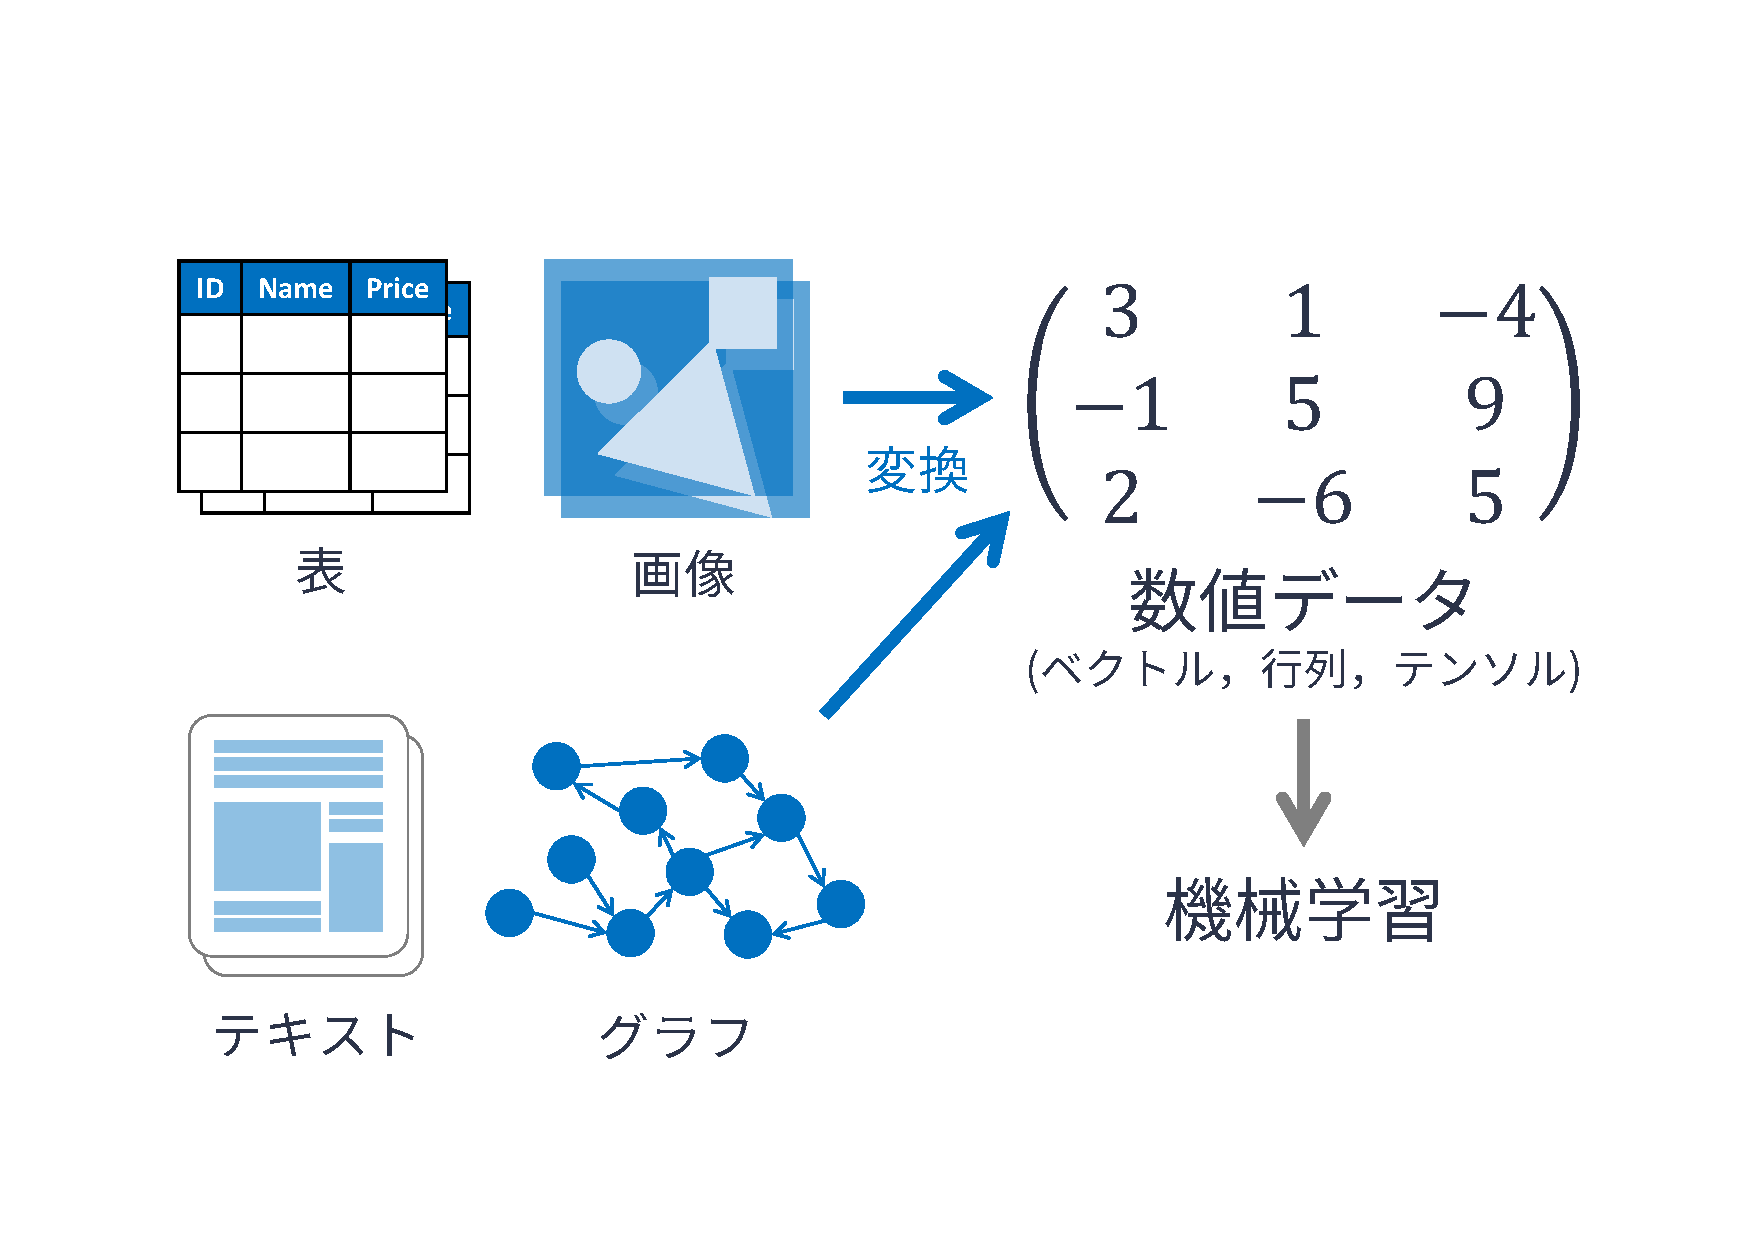
\includegraphics[width=0.75\textwidth]{figure/design-and-analysis-example/to-numerical-data.pdf}
    \caption{機械学習のための数値データ変換．}
    \label{fig:to-numerical-data}
\end{figure}

ところが，データベースから抽出した直後のデータには，文字列データやスケールの異なる数値など，すぐには数値として扱えないデータが多数含まれています．
また，統計モデリングや機械学習といったデータ分析手法の性能を引き出すために，より高度な統計処理を適用してデータを加工する必要もあります．
このような問題を解消するために，データ分析手法の適用に先立って\strong{前処理（Data Wrangling）}と呼ばれる作業を行います．
一般に，データ分析や機械学習のプロジェクトにおいて，前処理にかかる時間と労力は全体の8割を占めると言われています（残りの2割が分析手法の適用と評価です）．

こうした複雑で柔軟な対応が求められる前処理作業は，データベース言語であるSQLだけで完結させるのは非常に困難です．
そこで登場するのが，プログラミング言語を用いたデータ処理です．
現在，データサイエンスの世界で事実上の標準言語となっているPythonと，その強力なデータ分析ライブラリである\strong{pandas}を活用することで，データ分析の「前処理」の問題を柔軟に解決することができます．
pandasは行列データを効率的に扱うNumPyライブラリをベースに実装されていることもあり，機械学習ライブラリとの相性が良いです．
実際，機械学習のためのライブラリとして最も有名なscikit-learnは，pandasのデータフレーム（後述）を直接入力として受け取ることができます．

本章では，関係データベースから抽出したデータをPythonのpandasで処理し，より高度なデータ分析や機械学習へとつなぐための最低限のテクニックを速習します．
SQLとpandasを組み合わせることで，データベースを起点とした一連のデータ分析フローを一通りできるようになることが本章のゴールです．
pandasの詳しい使い方や様々な前処理テクニックについては，公式ドキュメント\footnote{pandas公式ドキュメント: \url{https://pandas.pydata.org/docs/}}や参考書\cite{前処理大全}などを参照してください．

\begin{notebox}{pandasの読み方と由来}
pandasは「パンダス」と読みます．動物のパンダとは直接の関係はなく，その名前はPythonによるデータ解析（\textit{Python Data Analysis}）を略した造語に由来するという説や，計量経済学で用いられる多次元データ「パネルデータ（\textit{panel data}）」に由来するという説が有力です．
\end{notebox}

% ==============================================================
\section{SQLとpandasの役割分担}
% ==============================================================
前処理の具体的なテクニックを見る前に，なぜSQLだけでなくpandasを学ぶ必要があるのか，その役割分担について整理しておきましょう．

SQLは，関係データベースという「巨大なデータの倉庫」の中で，条件に合うデータを探し出したり，基本的な集計を行ったりするのに特化しています．
一方，pandasは，取り出したデータを手元の計算機のメモリ上に展開し，Pythonの柔軟なプログラミング機能を駆使して「データを加工・変換する」ことに特化しています．
この特徴を踏まえた，SQLとpandasの具体的な役割分担は以下の通りです：
\begin{itemize}
    \item \strong{SQL：} 大規模データからの高速な絞り込み，テーブル同士の結合，単純な集計（売上合計など）．
    \item \strong{pandas：} 欠損値（空欄）の高度な穴埋め，文字列の複雑な加工，機械学習向けのデータ変換，他ライブラリ（グラフ描画やAIモデル）との連携．
\end{itemize}

実際のデータ分析プロジェクトでは，「\strong{SQLで必要なデータを絞り込んで抽出し，pandasで統計モデリングや機械学習用に加工する}」というのが典型的なワークフローとなります．
数億件のデータをいきなりpandasで読み込もうとすると，PCのメモリがパンクしてしまいます．
データベース側でできる絞り込みはSQLに任せ，複雑な処理だけをpandasで行うという役割分担を意識しましょう．

% ==============================================================
\section{DataFrame（データフレーム）とは}
% ==============================================================
pandasの中心となる概念が\strong{DataFrame（データフレーム）}です．
データフレームは，ExcelやGoogleスプレッドシートの「シート」に相当するもので，行と列からなる2次元の表形式データを扱うためのデータ構造です．

関係データベースの「テーブル（表）」と非常に似ていますが，Pythonのプログラム上で柔軟に操作できる点が特徴です．
関係データベースとpandasの用語の対応関係を表\ref{tab:pandas-df-vs-table}にまとめました．

\begin{table}[!htbp]
    \centering
    \caption{関係データベースのテーブルとデータフレームの用語の比較}
    \begin{tabular}{ll}
    \toprule
    \textbf{関係データベースのテーブル} & \textbf{pandasのデータフレーム} \\ \midrule
    テーブル（表）       & DataFrame（データフレーム） \\
    行（レコード / タプル）       & 行（row）\\
    列（カラム / 属性）         & 列（column）\\
    %列（カラム / 属性）         & 列（column / series）\\
    主キー               & インデックス（index）\footnote{pandasのインデックスは，関係データベースの主キーのような制約を自動的には保証しません}\\ \bottomrule
    \end{tabular}
    \label{tab:pandas-df-vs-table}
\end{table}

% データフレームから「1つの列だけ」を取り出したものは，\strong{Series（シリーズ）}と呼ばれる1次元のデータ構造になります．
% データフレームは「Seriesの集まり」でできていると考えると理解しやすいでしょう．

% ==============================================================
\section{分析環境の準備とデータの読み込み}
% ==============================================================
それでは，実際にpandasを使ってみましょう．
本章でも，これまでの章で用いてきた小売店ショッピングサイトの仮想データベース（\graybox{sql2-example.db}）を使用します．

\subsection{ライブラリのインストールとインポート}\label{sec:pandas-install}
まずは，pandasに加え，データベース接続に必要となるSQLAlchemy，データの前処理・機械学習を行うためのscikit-learnというライブラリをインストールします．
これらライブラリのインストールが完了していない場合は，ターミナルでコード\ref{code:pandas-install}のコマンドを実行してインストールしてください．

\begin{figure}[!htbp]
    \begin{minted}[gobble=1,
        bgcolor=background,
        fontsize=\small,
        linenos=false,
        xleftmargin=0em]{bash}

    pip install pandas sqlalchemy scikit-learn

    \end{minted}
    \captionsetup{name=コード}
    \caption{pandas，SQLAlchemy，およびscikit-learnのインストール}
    \label{code:pandas-install}
\end{figure}

インストールが完了したら，Pythonのスクリプト（またはJupyter Notebook）の先頭でこれらをインポートし，データベースへの接続準備を行います．
コード\ref{code:pandas-import}は，\graybox{sql2-example.db}ファイルに格納された関係データベースに接続する準備を行うためのコードです．
慣習として，pandasは\graybox{pd}という短い別名をつけてインポートします．
\graybox{create\_engine}は，データベースへの接続情報を管理するオブジェクトを作成する関数です．

\begin{figure}[!htbp]
    \begin{minted}[gobble=1,
        bgcolor=background,
        fontsize=\small,
        linenos=false,
        xleftmargin=0em]{python}

    import pandas as pd
    import sqlalchemy

    # SQLiteデータベースへの接続エンジンを作成する
    db_path = 'sql2-example.db'
    engine = sqlalchemy.create_engine(f'sqlite:///{db_path}')

    \end{minted}
    \captionsetup{name=コード}
    \caption{ライブラリのインポートと関係データベースへの接続}
    \label{code:pandas-import}
\end{figure}

\subsection{SQLを発行してデータフレームを作成する}\label{sec:pandas-read-sql}
準備が整ったら，データベースにSQLクエリを発行し，その結果をそのままデータフレームとして受け取ってみましょう．
使用するのは\graybox{pd.read\_sql()}関数です．

\begin{figure}[!htbp]
    \begin{minted}[gobble=1,
        bgcolor=background,
        fontsize=\small,
        linenos=false,
        xleftmargin=0em]{python}

    # 「商品」テーブルの全レコードを取得する
    sql = 'SELECT * FROM 商品;'
    df_products = pd.read_sql(sql, engine)

    \end{minted}
    \captionsetup{name=コード}
    \caption{\texttt{read\_sql()}によるデータベースからの読み込み}
    \label{code:pandas-read-sql}
\end{figure}

\graybox{read\_sql()}関数は，第1引数に実行したいSQL文，第2引数に接続エンジンを指定することで，SQL文による問い合わせ結果をPythonのデータフレームに変換してくれます．
単なる全件取得だけでなく，\graybox{JOIN}や\graybox{GROUP BY}を含む複雑なSQL文を渡せるため，たった数行のコードを書くだけで，データベースへの問い合わせ結果をPython側に取り込むことができます．

コード\ref{code:pandas-read-sql}は，\graybox{sql2-example.db}ファイルに格納された関係データベースにSQL文を発行し，「商品」テーブルの全レコードをデータフレームとして変数\graybox{df\_products}に格納する例です．
\graybox{df\_products}の先頭5件は，図\ref{fig:pandas-read-sql-results}のような内容となります．

\begin{figure}[!htbp]
    \centering
    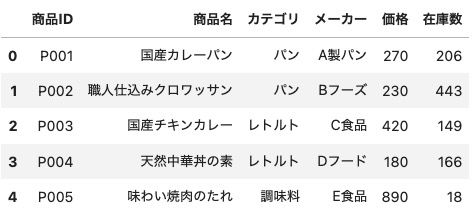
\includegraphics[width=0.80\textwidth]{figure/pandas/pandas-read-sql-results.jpg}
    \caption{\graybox{df\_products}の先頭5件．}
    \label{fig:pandas-read-sql-results}
\end{figure}

なお，今回の例では関係データベースシステムとしてSQLiteを使うことを想定していますが，MySQLやPostgreSQLなど他の関係データベースシステムを用いる場合も，同様に\graybox{pandas.read\_sql}関数を使うことができます．
このように，pandasは「データベースと機械学習をつなぐ接点」となります．

% ==============================================================
\section{データフレームの基本操作}
% ==============================================================
データを読み込んだら，その全体像を把握することがデータ分析の第一歩です．

\subsection{データの概要確認}
コード\ref{code:pandas-overview}に記したいくつかのメソッドを使うことで，読み込んだデータフレームのサイズや列の構成，欠損値（空欄）の有無をすばやく確認できます（実行結果\ref{fig:pandas-overview-results}参照）．
特に\graybox{info()}メソッドは重要です．
各列のデータの型（文字が入っているのか，数値が入っているのか等）や，データが欠損している行の数を一目で把握できます．
データの前処理を始める前に，必ず実行する習慣をつけましょう．

\begin{figure}[!htbp]
    \begin{minted}[gobble=1,
        bgcolor=background,
        fontsize=\small,
        linenos=false,
        xleftmargin=0em]{python}

    df_products.shape        # データフレームの行数と列数を返す
    df_products.columns      # 列名の一覧を返す
    df_products.info()     # 列ごとのデータ型と非NULL値の数を表示する
    df_products.describe()   # 数値列の基本統計量（平均，最大値など）を表示する

    \end{minted}
    \captionsetup{name=コード}
    \caption{データフレームの概要の確認}
    \label{code:pandas-overview}
\end{figure}

\begin{figure}[!htbp]
    \centering
    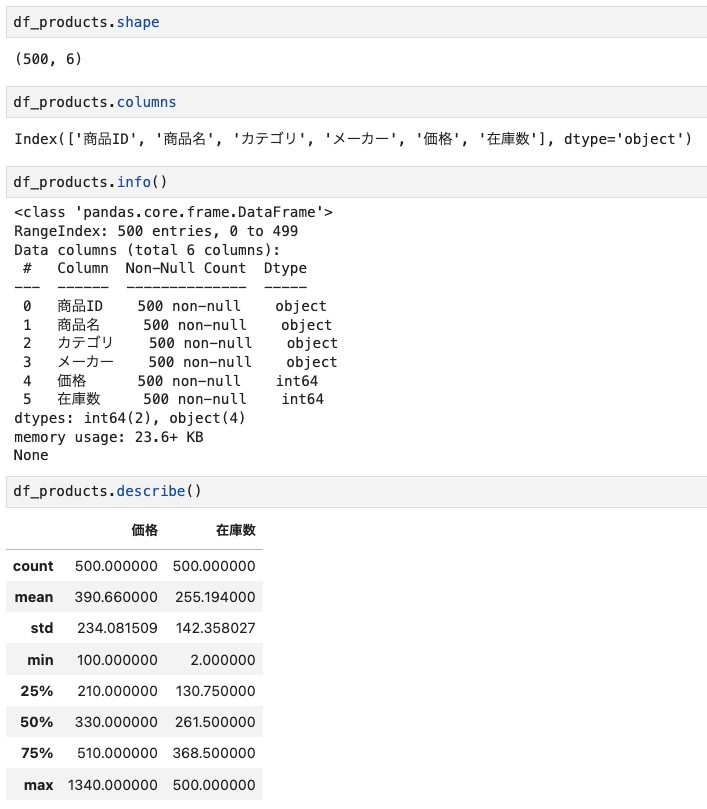
\includegraphics[width=0.99\textwidth]{figure/pandas/pandas-overview-results.jpg}
    \caption{コード\ref{code:pandas-overview}の実行結果}
    \label{fig:pandas-overview-results}
\end{figure}


\subsection{列の参照と行の絞り込み}
SQLの\graybox{SELECT 列名}に相当する，特定の列の情報を抽出する操作は，コード\ref{code:pandas-column-select}のようにデータフレームに対して角括弧\graybox{[]}を使って行います．
図\ref{fig:subset_df}は，コード\ref{code:pandas-column-select}で新しく作成したデータフレーム\graybox{subset\_df}の先頭5件です．

\begin{figure}[!htbp]
    \begin{minted}[gobble=1,
        bgcolor=background,
        fontsize=\small,
        linenos=false,
        xleftmargin=0em]{python}

    # 1つの列だけを取り出す
    names = df_products['商品名']

    # 複数の列を取り出す
    subset_df = df_products[['商品名', '価格', 'カテゴリ']]

    \end{minted}
    \captionsetup{name=コード}
    \caption{列の参照}
    \label{code:pandas-column-select}
\end{figure}

\begin{figure}[!htbp]
    \centering
    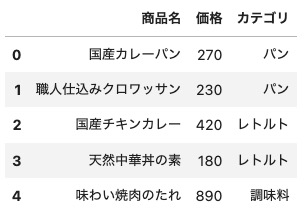
\includegraphics[width=0.55\textwidth]{figure/pandas/subset_df.jpg}
    \caption{\graybox{subset\_df}の先頭5件．}
    \label{fig:subset_df}
\end{figure}


SQLの\graybox{WHERE}句に相当する行の絞り込みを行うには，コード\ref{code:pandas-filter}のように角括弧\graybox{[]}の中に条件式を指定するか，\graybox{query}メソッドを使って記述します．
図\ref{fig:pandas-filter-results}は，コード\ref{code:pandas-filter}で新たに作成されたデータフレームの先頭5件を表示したものです．

\begin{figure}[!htbp]
    \begin{minted}[gobble=1,
        bgcolor=background,
        fontsize=\small,
        linenos=false,
        xleftmargin=0em]{python}

    # 価格が500円以上の商品を絞り込む
    expensive_items = df_products[df_products['価格'] >= 500]

    # 文字列の条件検索：商品名に「カレー」が含まれるものを探す
    curry_items = df_products[df_products['商品名'].str.contains('カレー')]

    # query()メソッドを使うとSQLライクに書けて読みやすい
    expensive_seasonings = df_products.query('価格 >= 500 & カテゴリ == "調味料"')

    \end{minted}
    \captionsetup{name=コード}
    \caption{行の絞り込み}
    \label{code:pandas-filter}
\end{figure}

\begin{figure}[!htbp]
    \centering
    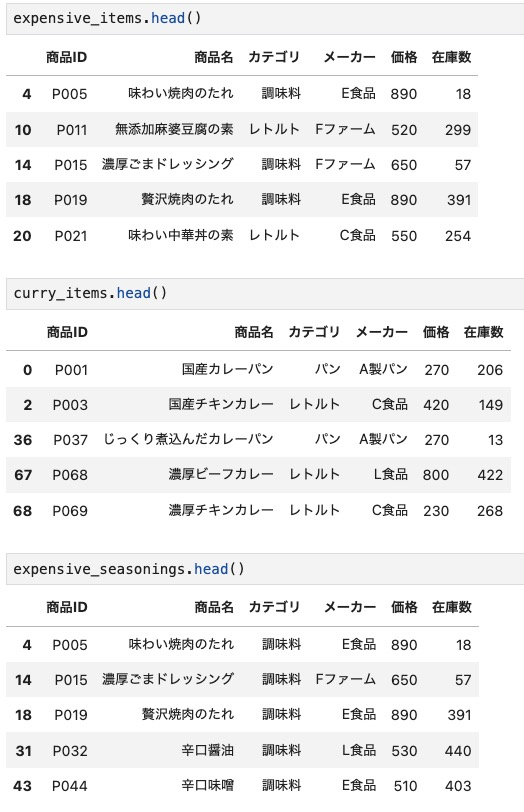
\includegraphics[width=0.80\textwidth]{figure/pandas/pandas-filter.jpg}
    \caption{コード\ref{code:pandas-filter}で新たに作成されたデータフレームの先頭5件．}
    \label{fig:pandas-filter-results}
\end{figure}

% ==============================================================
\section{データの加工と集計}
% ==============================================================
分析を進める中で，新しい指標（列）を作ったり，特定の条件で集計し直したりする場面が多々あります．
pandasでデータの加工や集計を行う方法を確認しておきましょう．

\subsection{新しい列の追加と計算}
コード\ref{code:pandas-new-column}のように代入演算を用いることで，データフレームに新しい列を追加したり，既存の列を使った計算結果を新しい列として格納したりすることができます．
図\ref{fig:pandas-new-column-results}は，コード\ref{code:pandas-new-column}を実行することで新たな列が追加された\graybox{df\_products}の先頭5件を表示したものです．

\begin{figure}[!htbp]
    \begin{minted}[gobble=1,
        bgcolor=background,
        fontsize=\small,
        linenos=false,
        xleftmargin=0em]{python}

    # 「価格」と「在庫数」を掛けて，「在庫金額」という新しい列を作る
    df_products['在庫金額'] = df_products['価格'] * df_products['在庫数']

    \end{minted}
    \captionsetup{name=コード}
    \caption{列の追加と計算}
    \label{code:pandas-new-column}
\end{figure}

\begin{figure}[!htbp]
    \centering
    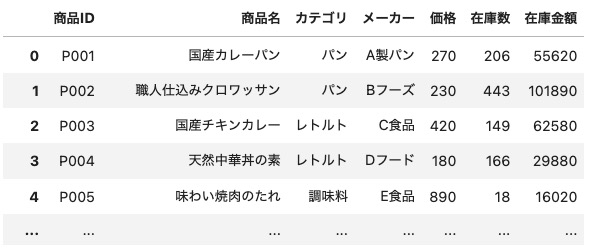
\includegraphics[width=0.80\textwidth]{figure/pandas/pandas-new-column-results.jpg}
    \caption{コード\ref{code:pandas-new-column}で新たに列が追加された\graybox{df\_products}の先頭5件．}
    \label{fig:pandas-new-column-results}
\end{figure}


\subsection{関数の適用}
各行の値に対して独自の複雑な処理を行いたい場合は，\graybox{apply()}メソッドを使います．
これにより，自分で定義した関数を列全体に一括で適用できます．
コード\ref{code:pandas-apply}は，列「価格」の値に応じて価格帯のカテゴリを割り振るためのコード例です．
図\ref{fig:pandas-apply-results}は，コードを実行した後に得られる\graybox{df\_products}の先頭5件を表示したものです．

\begin{figure}[!htbp]
    \begin{minted}[gobble=1,
        bgcolor=background,
        fontsize=\small,
        linenos=false,
        xleftmargin=0em]{python}

    # 価格に応じて3段階のカテゴリに分類する関数
    def classify_price(p):
        if p >= 500:
            return '高価格'
        elif p >= 300:
            return '中価格'
        else:
            return '低価格'

    # applyメソッドで関数を列全体に適用する
    df_products['価格帯'] = df_products['価格'].apply(classify_price)

    # ラムダ式（無名関数）を使って1行で簡潔に書くこともできる
    # 例：500円以上の商品だけを1割引きにする
    df_products['割引後価格'] = df_products['価格'].apply(
        lambda p: p * 0.9 if p >= 500 else p
    )

    \end{minted}
    \captionsetup{name=コード}
    \caption{\texttt{apply()}による関数の適用}
    \label{code:pandas-apply}
\end{figure}

\begin{figure}[!htbp]
    \centering
    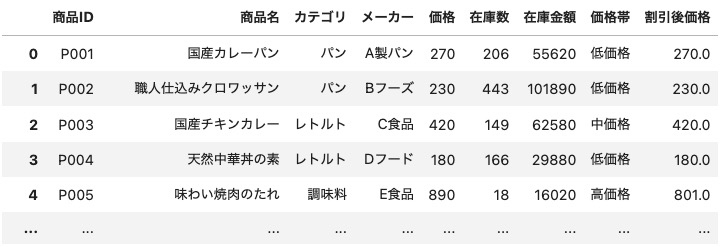
\includegraphics[width=0.95\textwidth]{figure/pandas/pandas-apply-results.jpg}
    \caption{コード\ref{code:pandas-apply}で新たに列が追加された\graybox{df\_products}の先頭5件．}
    \label{fig:pandas-apply-results}
\end{figure}

\subsection{グループ化と集計}
SQLの\graybox{GROUP BY}と同じように，特定のカテゴリごとにデータをまとめて集計するには\graybox{groupby()}メソッドを使用します（コード\ref{code:pandas-groupby}参照）．
図\ref{fig:pandas-groupby-results}はコード\ref{code:pandas-groupby}を実行した結果，得られたデータフレームの中身を表示したものです．

\begin{figure}[!htbp]
    \begin{minted}[gobble=1,
        bgcolor=background,
        fontsize=\small,
        linenos=false,
        xleftmargin=0em]{python}

    # カテゴリごとの在庫数の合計を計算する
    stock_sum = df_products.groupby('カテゴリ')[['在庫数']].sum()

    # カテゴリごとの価格の平均と最大値を一度に計算する
    price_stats = df_products.groupby('カテゴリ').agg({'価格': ['mean', 'max']})

    \end{minted}
    \captionsetup{name=コード}
    \caption{\texttt{groupby()}による集計}
    \label{code:pandas-groupby}
\end{figure}

\begin{figure}[!htbp]
    \centering
    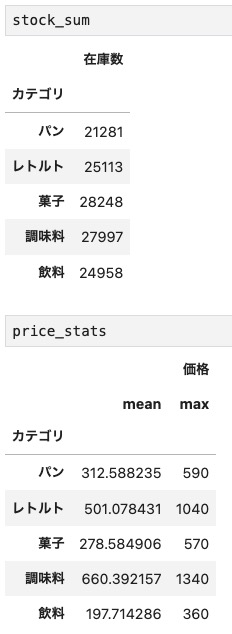
\includegraphics[width=0.35\textwidth]{figure/pandas/pandas-groupby-results.jpg}
    \caption{コード\ref{code:pandas-groupby}の実行後に得られる\graybox{stock\_sum}および\graybox{price\_stats}．}
    \label{fig:pandas-groupby-results}
\end{figure}

また，特定の値の出現頻度（そのカテゴリの商品がいくつあるか等）を数えたい場合は，コード\ref{code:pandas-value-counts}のように\graybox{value\_counts()}が便利です．
図\ref{fig:pandas-value-counts-results}はコード\ref{code:pandas-value-counts}の実行結果です．

\begin{figure}[!htbp]
    \begin{minted}[gobble=1,
        bgcolor=background,
        fontsize=\small,
        linenos=false,
        xleftmargin=0em]{python}

    # カテゴリごとの商品数を数える
    df_products['カテゴリ'].value_counts()

    \end{minted}
    \captionsetup{name=コード}
    \caption{\texttt{value\_counts()}による頻度集計}
    \label{code:pandas-value-counts}
\end{figure}

\begin{figure}[!htbp]
    \centering
    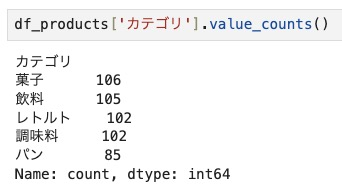
\includegraphics[width=0.60\textwidth]{figure/pandas/pandas-value-counts-results.jpg}
    \caption{コード\ref{code:pandas-value-counts}の実行結果．}
    \label{fig:pandas-value-counts-results}
\end{figure}

% ==============================================================
\section{データフレームの結合（縦と横）}
% ==============================================================
データ分析では，複数の表データを結合して1つのデータセットにまとめる作業が頻繁に発生します．
データフレーム同士を結合する方法を確認しておきましょう．

\subsection{横方向の結合（merge）}
SQLの\graybox{JOIN}に相当する操作が\graybox{merge()}です．
共通の列（キー）を使って，2つのデータフレームを横方向につなぎ合わせます．
コード\ref{code:pandas-merge}は，データフレーム\graybox{df\_orders}と\graybox{df\_products}を列「商品ID」の値をもとに結合するためのものです．
このコードを実行すると，図\ref{fig:pandas-merge-results}のようなデータフレーム\graybox{df\_merged}が得られます．
なお，\graybox{how}パラメータには，SQLと同様に\graybox{inner}（内部結合），\graybox{left}（左外部結合）などを指定できます．

\begin{figure}[!htbp]
    \begin{minted}[gobble=1,
        bgcolor=background,
        fontsize=\small,
        linenos=false,
        xleftmargin=0em]{python}

    # 注文テーブルを読み込む
    df_orders = pd.read_sql('SELECT * FROM 注文', engine)

    # 「商品ID」をキーにして，注文データに商品データを内部結合する
    df_merged = pd.merge(df_orders, df_products, on='商品ID', how='inner')

    \end{minted}
    \captionsetup{name=コード}
    \caption{\texttt{merge()}による横方向の結合}
    \label{code:pandas-merge}
\end{figure}

\begin{figure}[!htbp]
    \centering
    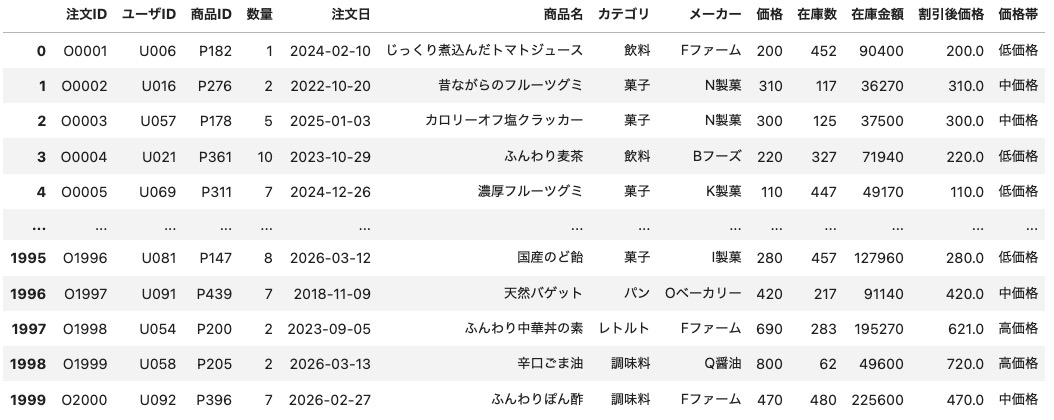
\includegraphics[width=0.999\textwidth]{figure/pandas/pandas-merge-results.jpg}
    \caption{コード\ref{code:pandas-merge}を実行した結果，得られるデータフレーム\graybox{df\_merged}．}
    \label{fig:pandas-merge-results}
\end{figure}

\subsection{縦方向の結合（concat）}
SQLの\graybox{UNION ALL}に近い操作が\graybox{concat()}です\footnote{SQLの\graybox{UNION}は重複を削除しますが，\graybox{concat()}は重複を保持します．重複排除が必要なら追加処理が必要となります．}．
同じ列構成を持つデータフレームを，縦に積み重ねます．
コード\ref{code:pandas-concat}は，2024年以前の注文に関するデータが収められたデータフレーム\graybox{df\_orders\_before\_2024}と2024年以降の注文データが格納された\graybox{df\_orders\_after\_2024}が与えられたときに，2つのデータフレームを積み重ねて1つのデータフレーム\graybox{df\_orders}にするためのコードです．
注意点としては，SQLの集合演算と同様，\graybox{concat}の対象となるデータフレームは列構造（列の順序も含む）が揃っている必要があります．

\begin{figure}[!htbp]
    \begin{minted}[gobble=1,
        bgcolor=background,
        fontsize=\small,
        linenos=false,
        xleftmargin=0em]{python}

    # 2024年以前の注文データと2024年以降の注文データを縦につなぐ
    # ignore_index=True を指定してインデックスを振り直す
    df_orders = pd.concat(
        [df_orders_before_2024, df_orders_after_2024], ignore_index=True)

    \end{minted}
    \captionsetup{name=コード}
    \caption{\texttt{concat()}による縦方向の結合}
    \label{code:pandas-concat}
\end{figure}

% ==============================================================
\section{機械学習のための前処理技法}
% ==============================================================
ここからがpandasの真骨頂です．
SQLで抽出・結合したデータを，機械学習モデルが理解できる形に変換する「前処理」テクニックの基礎を学びましょう．

\subsection{欠損値（NULL）の処理}
関係データベースで外部結合（LEFT JOIN）を行った際などに発生する欠損値\graybox{NULL}は，pandasでは\graybox{NaN}（Not a Number）として表現されます．
多くの機械学習モデルは欠損値が含まれていると計算エラーを起こしてしまうため，何らかの対処が必要です．
コード\ref{code:pandas-missing-values}は，欠損値が含まれる行を削除したり，特定の列に含まれる欠損値を別の値に置換したりするコードの例です．
SQLで2つのテーブルを外部結合して得られた\graybox{df\_merged}には，実は「数量」の値が\graybox{NaN}になっているレコードが2つ存在します．
コード\ref{code:pandas-missing-values}の最終行で穴埋めをすると，図\ref{fig:pandas-missing-values-results}のように\graybox{df\_merged}の中身が変更されます．

\begin{figure}[!htbp]
    \begin{minted}[gobble=1,
        bgcolor=background,
        fontsize=\small,
        linenos=false,
        xleftmargin=0em]{python}

    sql = """
    SELECT
        *
    FROM
        商品
    LEFT OUTER JOIN 注文
    USING(商品ID);
    """

    # 「商品」テーブルと「注文」テーブルを「商品ID」で外部結合したものをデータフレームに
    df_merged = pd.read_sql(sql, engine)

    # NaNが含まれる行をまるごと削除する（情報が失われるので注意）
    df_clean = df_merged.dropna()

    # NaNを特定の値（例えば0）で穴埋めする
    df_merged['数量'] = df_merged['数量'].fillna(0)

    \end{minted}
    \captionsetup{name=コード}
    \caption{欠損値の処理}
    \label{code:pandas-missing-values}
\end{figure}

\begin{figure}[!htbp]
    \centering
    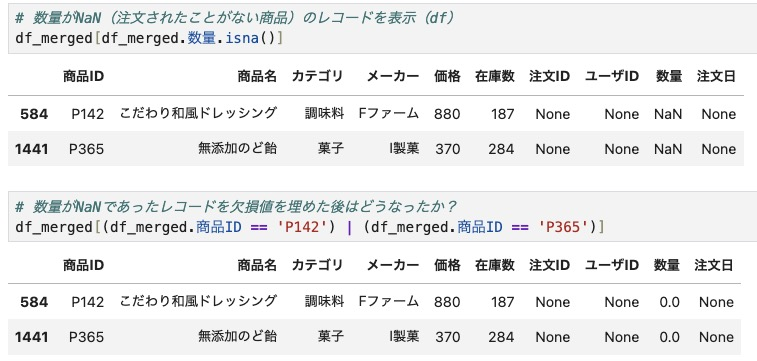
\includegraphics[width=0.99\textwidth]{figure/pandas/pandas-missing-values-results.jpg}
    \caption{コード\ref{code:pandas-missing-values}を実行した結果，\graybox{df\_merged}の一部が穴埋めされる．}
    \label{fig:pandas-missing-values-results}
\end{figure}

\subsection{カテゴリ変数のダミー変数化}
機械学習モデルは原則「数値」しか理解できません．
「カテゴリ」列に入っている「パン」「レトルト」「調味料」といったカテゴリを示す文字列データは，そのままでは計算に使えません．

\begin{figure}[!htbp]
    \centering
    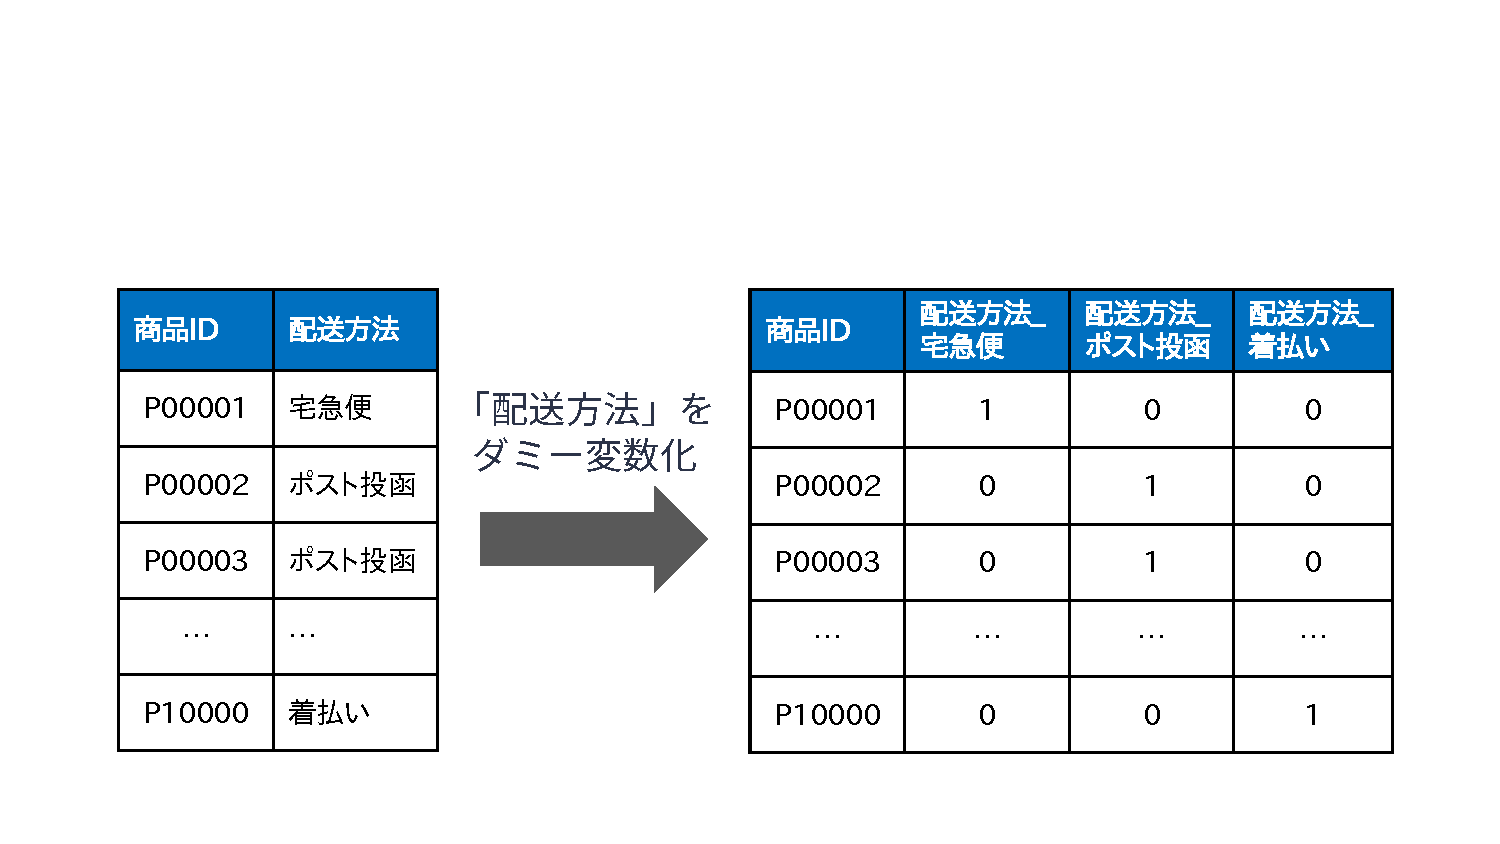
\includegraphics[width=0.85\textwidth]{figure/pandas/one-hot-encoding.pdf}
    \caption{カテゴリ変数のダミー変数化の例．}
    \label{fig:one-hot-encoding}
\end{figure}
一般にカテゴリを示すデータについては，図\ref{fig:one-hot-encoding}のように，カテゴリの数だけ新しい列（フラグ）を作り，該当する箇所に1，それ以外に0を入れる変換を行います．
これを\strong{ダミー変数化（またはワンホットエンコーディング; one-hot encoding）}と呼びます．
pandasでは\graybox{get\_dummies()}という関数でカテゴリ変数を数値に変換できます．
コード\ref{code:pandas-dummies}は，商品に関するデータフレームの列「カテゴリ」のデータをダミー変数化するためのコード例です．
このコードを実行すると，図\ref{fig:pandas-dummies-results}のようなデータフレームを得ることができます．
\begin{figure}[!htbp]
    \begin{minted}[gobble=1,
        bgcolor=background,
        fontsize=\small,
        linenos=false,
        xleftmargin=0em]{python}

    # 「カテゴリ」列をダミー変数化する
    df_encoded = pd.get_dummies(df_products, columns=['カテゴリ'], dtype='int')

    \end{minted}
    \captionsetup{name=コード}
    \caption{ダミー変数化のためのコード例}
    \label{code:pandas-dummies}
\end{figure}

\begin{figure}[!htbp]
    \centering
    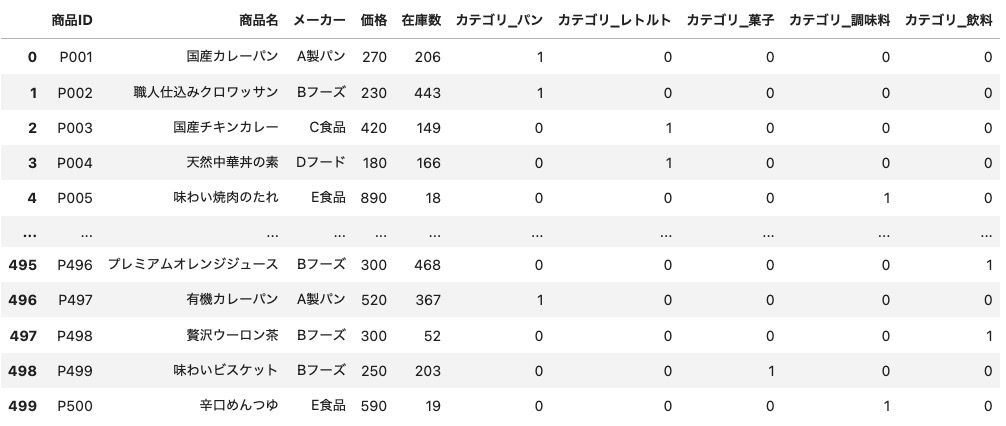
\includegraphics[width=0.99\textwidth]{figure/pandas/pandas-dummies-results.jpg}
    \caption{コード\ref{code:pandas-dummies}を実行した結果，得られた\graybox{df\_encoded}．}
    \label{fig:pandas-dummies-results}
\end{figure}

\subsection{数値のスケーリング}
データの中に「価格（数百円〜数十万円）」と「在庫数（数個〜数百個）」のように，桁（スケール）が全く違う変数が混ざっていると，機械学習の手法によっては「桁が大きいデータの方が重要だ」と勘違いしてしまうことがあります\footnote{距離ベースの手法や正則化を伴う線形モデルなどでは，スケールの影響を受けやすいです．}．
これを防ぐため，データのスケールを一定のルールで揃える「正規化」や「標準化」を行います．
正規化および標準化の数学的操作は以下の通りです：
\begin{itemize}
    \item \strong{正規化（normalization, min-max scaling）：} データが0から1の範囲に収まるように元データを変換．
    \begin{equation}
        x' = \frac{x - x_{\min}}{x_{\max} - x_{\min}}
        \label{eq:normalization}
    \end{equation}
    \item \strong{標準化（standardization）：} 平均が0，標準偏差が1になるように元データを変換．
    \begin{equation}
        x' = \frac{x - \mu}{\sigma}
        \label{eq:standardization}
    \end{equation}
\end{itemize}

これらの処理は直接計算することも可能ですが，機械学習ライブラリ\graybox{scikit-learn}の\graybox{MinMaxScaler}や\graybox{StandardScaler}を使うと，複数の列に対して効率的に適用できます．
コード\ref{code:pandas-sklearn-scaling}は，商品に関するデータフレームの列「価格」「在庫数」の値を正規化もしくは標準化するコード例です．
図\ref{fig:pandas-standardization-results}は，コード\ref{code:pandas-sklearn-scaling}の標準化の箇所を実行した結果得られるデータフレーム\graybox{df\_products}の中身となります．

\begin{figure}[!htbp]
    \begin{minted}[gobble=1,
        bgcolor=background,
        fontsize=\small,
        linenos=false,
        xleftmargin=0em]{python}

    from sklearn.preprocessing import MinMaxScaler, StandardScaler

    # 正規化（MinMaxScaler）
    # 価格と在庫数を正規化し，列の情報を更新
    scaler_minmax = MinMaxScaler()
    df_products[['価格_正規化', '在庫数_正規化']] = scaler_minmax.fit_transform(
        df_products[['価格', '在庫数']])

    # 標準化（StandardScaler）
    # 価格と在庫数を標準化し，新たな列を追加
    scaler_std = StandardScaler()
    df_products[['価格_標準化', '在庫数_標準化']] = scaler_std.fit_transform(
        df_products[['価格', '在庫数']])

    \end{minted}
    \captionsetup{name=コード}
    \caption{scikit-learnを用いたスケーリング}
    \label{code:pandas-sklearn-scaling}
\end{figure}

\begin{figure}[!htbp]
    \centering
    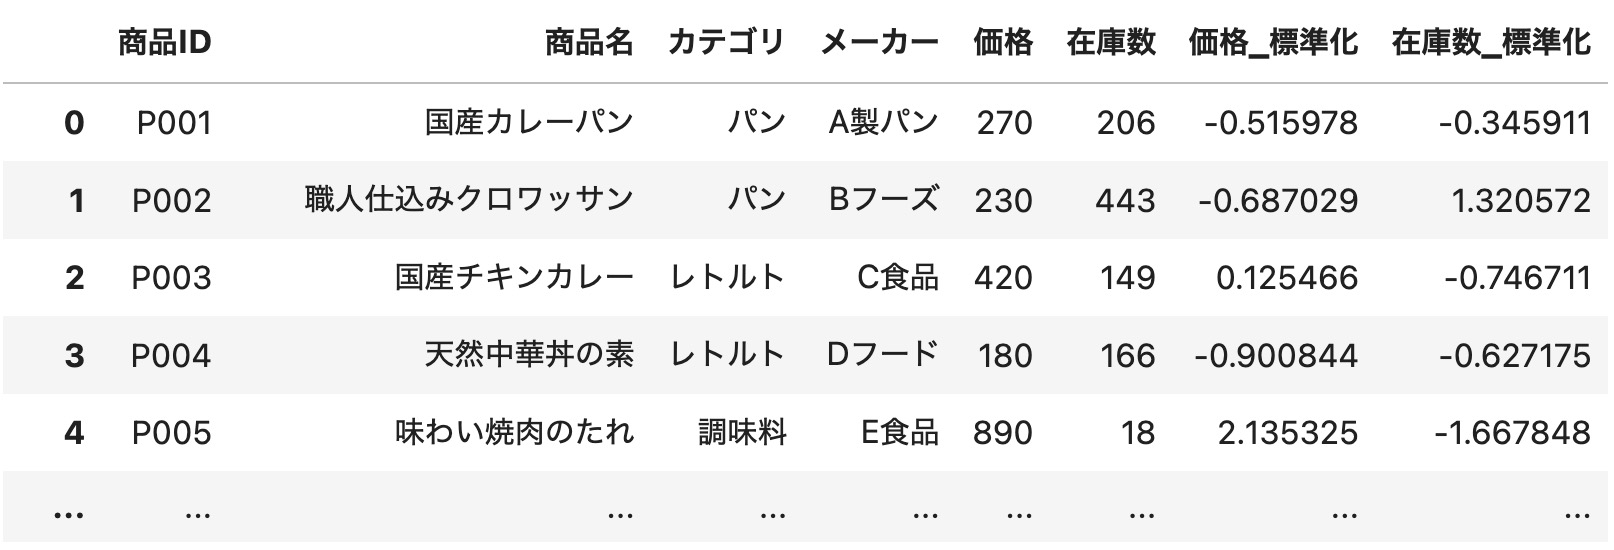
\includegraphics[width=0.99\textwidth]{figure/pandas/pandas-standardization-results.jpg}
    \caption{コード\ref{code:pandas-sklearn-scaling}によって「価格」列と「在庫数」列の値を標準化した結果，得られる\graybox{df\_products}．}
    \label{fig:pandas-standardization-results}
\end{figure}

% ==============================================================
\section{まとめ}
% ==============================================================
本章では，関係データベースのSQLとPythonのpandasを連携させ，データを機械学習モデルに投入可能な状態へと引き上げる「前処理」の基礎を学びました．

関係データベースを正しく設計し，SQLで必要なデータを効率よく抽出し，pandasでモデル向けに加工する ——
この一連の流れこそが，データ分析の実務そのものです．

次章では，これまでに学んだすべての知識（正規化設計，SQL，pandas）を総動員して，実践的なデータベースの設計・分析課題に挑みます．

